\newpage
\begin{song}{title={Pieśń wielorybników}, music={EKT Gdynia}}
\begin{multicols}{2}
    \begin{intro}   
        a a a d \\
        a e a a $\times 2$
    \end{intro}
    \begin{verse}
        Nasz D^{a}iament prawie g^{e}otów już \\
        W cieśn^{a}inach nie ma kr^{e}y \\
        Na k^{a}ei piękne pa^{e}nny stoją \\
        W ich o^{d}czach bły^{e}szczą ł^{a}zy \\
        Kapitan w niebo wlepia wzrok \\
        Ruszamy lada dzień \\
        Płyniemy tam, gdzie słońca blask \\
        nie mąci nocy cień 
    \end{verse}    
    \begin{chorus}
        A więc krz^{a}ycz: ^{e}o h^{a}o! \\
        Odw^{a}agę w s^{e}ercu mi^{a}ej \\
        Wielor^{a}ybów ci^{e}elska gr^{C}oźne s^{G}ą \\
        Lecz do^*{F}sta ni^{e}emy j^{a}e $\times 2$ \\ 
        
        a a a d \\
        a e a a $\times 2$
    \end{chorus}
    \begin{verse}
        Ej panno powiedz po co łzy \\
        Nic nie zatrzyma mnie \\
        Bo prędzej w wodach kwiat zakwitnie \\
        Niż wycofam się \\
        No nie płacz mała, wrócę tu \\
        Nasz los nie taki zły \\
        Bo da dukatów wór za tran \\
        I wielorybie kły
    \end{verse}
    \begin{chorus}
        A więc krzycz: o ho!\ldots $\times 2$
    \end{chorus}    
    \begin{verse}
        Na deku stary wąchał wiatr \\
        lunetę w ręku miał \\
        Na łodziach co zwisały już \\
        z harpunem każdy stał \\
        I dmucha tu i dmucha tam  \\
        ogromne stado w krąg \\
        Harpuny, wiosła, liny brać \\
        I ciągnij brachu ciąg
    \end{verse}
    \begin{chorus}
        A więc krzycz: o ho!\ldots $\times 2$
    \end{chorus} 
    \begin{verse}
    \textit{wolniej} \\
        I dla ^*{a}wielo ry^{G}ba j^{a}uż \\
        Ost^*{e} atn^{G}i to dz^{a}ień \\
        Bo śmi^{a}ały harp^*{C}u nn^{G}ik \\
        ^*{F}U de^{G}rza w^{a}eń \\ \\
        a a a d \\
        a e a a
    \end{verse}
\end{multicols}
\end{song}
\fancyfoot[LO,RE]{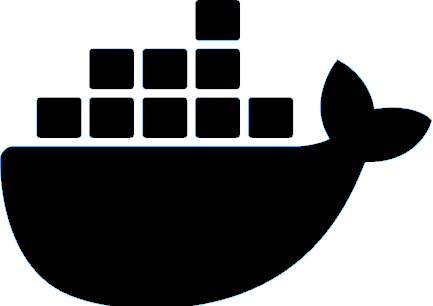
\includegraphics[height=45pt]{images/docker.png}}


